\section{Datenbank einrichten} \label{sec:database}
Bitte laden Sie nun die Datenbank herunter (mit dem Link aus der Einleitung) und entpacken Sie diese.
Wir nennen das entstehende Verzeichnis \texttt{datenbank}.
Laden Sie ebenfalls die Python-Codes herunter.
Führen Sie als erstes das Python-Skript \texttt{save\_eigenfaces.py} über die Kommandozeile (Linux, MacOS) oder über \href{https://ipython.org/install.html}{IPython} (Windows) aus und übergeben Sie dabei den Pfad zur Datenbank und einen Namen für das resultierende File (z.B. \texttt{eigenfaces.dat}), also
\begin{center}
\mintinline{python}{python3 save_eigenfaces.py datenbank eigenfaces.dat}
\end{center}
Dies generiert ein File \texttt{eigenfaces.dat} welches wir später brauchen um die Aufgaben zu lösen.
Damit lassen sich alle nachfolgenden Kapitel bearbeiten.
Alternativ kann man eine eigene Datenbank erstellen und stattdessen diese für die Bearbeitung des Lernskriptes verwenden.
Dieses Kapitel ist eine Anleitung dazu.
Es werden folgende Programme benötigt:
\begin{itemize}
	\item Ein Bildbearbeitungsprogramm wie zum Beispiel das open source Programm \href{https://www.gimp.org/}{GIMP}.
	\item Ein Tabellen-Kalkulationsprogramm wie zum Beispiel das open source Programm \href{https://de.libreoffice.org/discover/calc/}{LibreOffice Calc}.
\end{itemize}
Nehmen wir als Beispiel eine Schulklasse bestehend aus 10 Lernenden.
Jeder Schüler und jede Schülerin macht einige Fotos von seinem/ihrem Gesicht.
Sagen wir, 8 Fotos pro Person.
Das Ziel ist ein Verzeichnis \texttt{datenbank} anzulegen, welches wie in Abbildung~\ref{fig:database} aufgebaut ist.
\begin{figure}[ht]
	\centering
	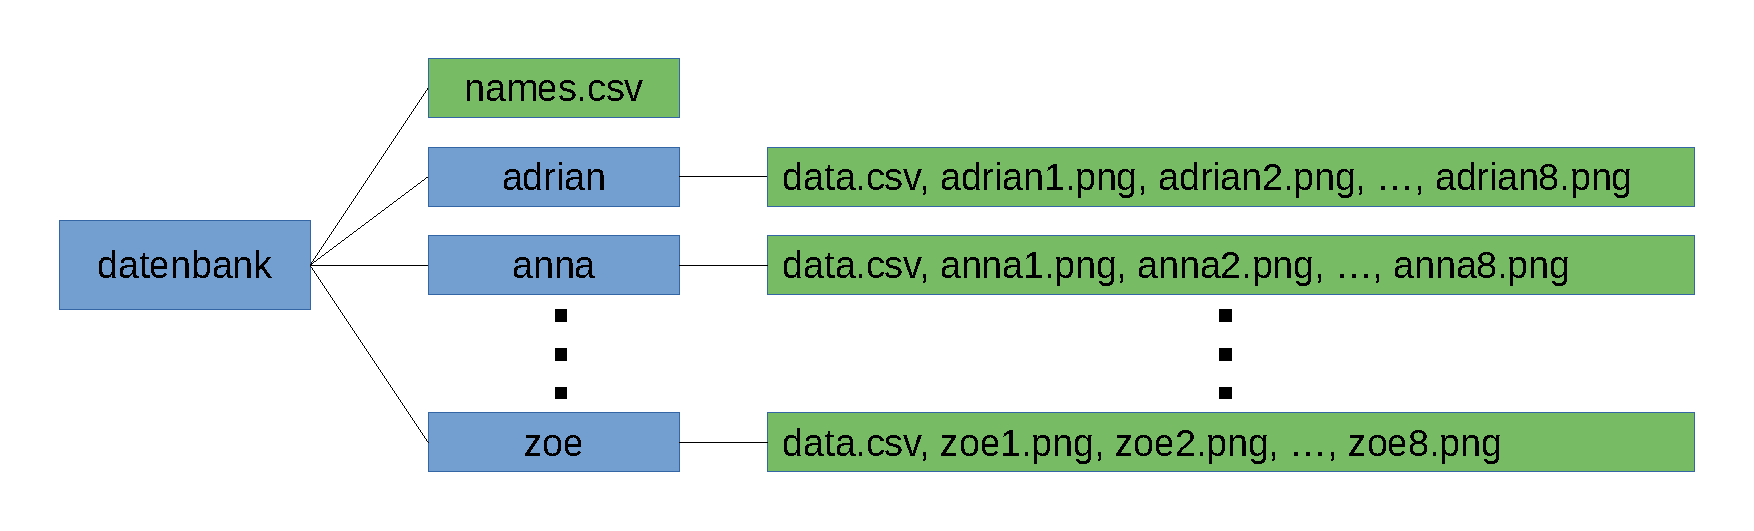
\includegraphics[width=\textwidth]{images/database}
	\caption{Datenbank aus Trainingsbildern. Die Verzeichnisse sind in blau und die Dateien in grün abgebildet.}
	\label{fig:database}
\end{figure}
Das heisst, pro Person enthält \texttt{datenbank} je ein Verzeichnis mit deren Namen.
Diese Verzeichnisse enthalten wiederum die 8 Fotos der jeweiligen Person.
Die Dateien mit der Endung \texttt{.csv} enthalten jeweils eine Tabelle und können mit einem Tabellenkalkulationsprogramm erstellt/editiert werden.
\begin{itemize}
	\item \texttt{names.csv}: Besteht aus 10 Zeilen, welche die 10 Unterverzeichnisse \texttt{adrian, anna, ..., zoe} von \texttt{datenbank} auflisten.
	Unser Programm benötigt dieses File um die Unterverzeichnisse zu finden.
	\item \texttt{data.csv}: Besteht aus 8 Zeilen, welche die Dateinamen der 8 Fotos auflisten.
	Zum Beispiel enthält \texttt{adrian/data.csv} die Zeilen \texttt{adrian1.png, adrian2.png, ..., adrian8.png}.
	Unser Programm benötigt dieses File um die Bilddateien in den Unterverzeichnissen zu finden.
\end{itemize}
Es fehlt noch ein letzter Schritt.
Die Bilder müssen noch in ein geeignetes Format gebracht werden.
Dazu verwenden wir ein Bildbearbeitungsprogramm.
\begin{itemize}
	\item Alle Bilder müssen auf die selbe Auflösung zugeschnitten werden.
	Eine geeignete Auflösung ist zum Beispiel eine Breite von $N=144$ Pixel und eine Länge von $M=180$ Pixel.
	\item Der vorherige Punkt sollte so bewerkstelligt werden, dass das Gesicht möglichst das ganze Bild ausfüllt.
	\item Alle Bilder müssen in ein schwarz-weiss Bild konvertiert werden.
\end{itemize}
Führen Sie dann die Schritte zu Beginn dieses Kapitels für diese Datenbank aus.
